%\documentclass[twocolumn]{article}
\documentclass[./exercises.tex]{subfiles}
\begin{document}

\textit{\textbf{Inlämning 1  } }
\begin{enumerate}
\item Förklara med hjälp av en skiss vad det innebär att månen spänner en halv grad\\
\begin{figure}[H]
\centering
\usetikzlibrary {calc}
\begin{tikzpicture}[ baseline={(0,0)}]
%\draw (0,0) grid (4,4);
% x-axis
\draw [thick,-] (0,2) -- (4,2.5);
\draw [thick,-] (0,2) -- (4,1.5);

  \coordinate   (A) at (4,2);
  \coordinate  (B) at (4,2.5);

  \draw (A) let
              \p1 = ($ (B) - (A) $)
            in
              circle ({veclen(\x1,\y1)});

  
  \pgfpathmoveto{\pgfpointorigin}
   \pgfpathmoveto{\pgfpoint{0cm}{1cm}}
  \pgfpathmoveto{\pgfpoint{1cm}{1.5cm}}
  \pgfpatharc{-90}{90}{.5cm}
  \pgfusepath{draw}
  \node[ right] at (1.5,2) {$\alpha=0.5^o$};
  \node at (4,1){Månen};

\end{tikzpicture}
\label{fig1}
\caption{Reflekterade strålar från månens kontur}
\end{figure}
Bilden söker illustrera reflekterade ljusstrålar från månens kontur till observatör på jorden bildar vinken
$\alpha \approx 0.5^o$.

\item Vilket avstånd måste en person hålla ett 2-euro mynt (med en diameter på 2,6 cm) för att det
ska spänna en vinkel av
\begin{enumerate}[label=(\alph*)]
\item 1 grad\\
\begin{flalign*}
d&=2.6 \text{ cm}\\
\alpha &= 1^o=\frac{1\cdot\pi}{180}=\frac{\pi}{180}\text{ rad}\\
D&=\frac{d}{\alpha}=\frac{2.6\cdot 180}{\pi}\approx 150 \text{ cm}\\
\end{flalign*}

\item 1 arcminut\\
\begin{flalign*}
d&=2.6 \text{ cm}\\
\alpha &= 1'=\frac{1}{60}\text{ deg}=\frac{1}{60}\frac{\pi}{180}\text{ rad}\\
D&=\frac{d}{\alpha}=\frac{2.6}{\frac{1}{60}\frac{\pi}{180}}=\frac{2.6\cdot 60\cdot 180}{\pi}\\
 &\approx 8938 \text{ cm} =8.9\text{ m}\\
\end{flalign*}

\item 1 arcsekund\\
\begin{flalign*}
d&=2.6 \text{ cm}\\
\alpha &= 1''=\frac{1}{60\cdot 60}\text{ deg}=\frac{1}{3600}\frac{\pi}{180}\text{ rad}\\
D&=\frac{d}{\alpha}=\frac{2.6}{\frac{1}{3600}\frac{\pi}{180}}=\frac{2.6\cdot 3600\cdot 180}{\pi}\\
 &=536288.5 \text{ cm}\approx 536 \text{ m}\\
\end{flalign*}
\end{enumerate}

\item Hur är en astronomisk enhet de nierad? Ge
ett exempel på när den här enheten kan vara användbar.\\

1 astronomisk enhet (AU) är medelavståndet mellan jorden och solen
$1.496\cdot 10^8$ km (medelvärdet av jordbaneradien).\\
Då vinkelavståndet till en himlakropp är en bågsekund och kroppens bredd
är en 1 AU så är avståndet till kroppen 1 parsec (3.26 ly).\\
För en betraktare ute i unversum på 1 parsec avstånd till jorden är vinkelavståndet för denne mellan
solen och jorden som störst 1 bågsekund. Planeterna ligger några AU från varandra. Närmsta
stjärnan ligger på ca 1 parsec avstånd (Proxima Centauri) och närmsta stjärnorna
ligger på  några parsec avstånd från varandra\footnote{Föreläsning två andra delen,Prof. Nils Ryde}


\item Astronomer använder tiopotenser för att beskriva anståndet till objekt. Säg ett objekt eller plats som är grovt/
ungefärligt placerat vid dessa olika avstånd\\

\begin{enumerate}[label=(\alph*)]
\item $10^2$ m\\
100 meter är kortaste sprintdistansen utomhus och minimum längden på en internationellt godkänd fotbollsplan (tror jag).
I runda slängar menar astronomer i princip alla avstånd som kan skrivas $n\cdot 10^2$ där $n$ är ett heltal och
$1\leq n \leq 9$

\item $10^0$ m\\
1 meter - längden på mitt skrivbord. En astronom menar här allt från 1 till 9 meter.

\item $10^1$ m \\
10 meter - I Helsinborg gäller\footnote{\url{https://helsingborg.se/trafik-och-stadsplanering/parkering/parkeringsregler-lathund/parkeringsregler-i-korsning/}} att
ett fordon inte får stannas eller parkeras i en vägkorsning
eller inom ett avstånd av 10 meter från en korsande körbanas närmaste ytterkant!
Men kan alltså betyda 90 meter i astronomers fikarum!

\item $10^3$ m\\
Det är ca 1 km från Hjulstabrons(Enköping) norra brofäste över till Märsön på väg 55.

\item $10^7$ m\\
Jordens diameter är ca $10^7$ meter

\item $10^{10}$ m\\
Ca 10 sådana avstånd är en jordbaneradien.

\item $10^{20}$ m\\
Man har uppskattat Vintergatans diameter till $10^{21}$ meter så det får plats 10 stycken sådana avstånd
på den diametern.
\end{enumerate}

\item Varför färdas stjärnor över
himlavalvet, samt varför ser vi olika stjärnor på himlen under olika tider av året (sommaren och
vintern)?\\

Stjärnorna är stationära relativt den tänkta himlasfären (hur detta går ihop med universums expansion förstår jag dock inte) och eftersom
jorden roterar runt solen så kommer vi att se stjärnorna från olika vinklar. 
Eftersom jorden rotererar (i högerbandens fingrars riktning då tummen pekar mot nordpolen) så kommer vi att se stjärnor gå
upp i öst och ner i väst. Lutningen på jordens rotationsaxel($23.5^o$) gör att stjärnorna för oss på norra halvklotet kommer komma upp längs en bågformad bana med vinkel mindre
än 90 grader mot horisonten nå en högsta punkt och sedan gå ner i en bågformad bana i väster.
Ju närmare ekvatorn vi kommer desto mer närmar sig vinkeln mot horistontalplanet för stjärnbildsbanorna $90^o$.Vänd mot väster
så kommer stjärnorn kommaupp bakom ryggen och gå ner i lodräta banor mot horisonten och vid nordpolen tittandes söder ut så kommer
stjärnorna dra förbi i horisontella banor från vänster(öster) till höger (väster). På samma sätt förhåller det sig det med vår stjärna
solen.

De stjärnor vars ljus når ögat tillsammans med solens strålar dränks av solljuset och är därför inte synliga och även om vi
kunnat detektera detta ljus så är ändå inte stjärnor som är skymda av solen synliga.
En stjärnbild som är helt skymd av solen blir därför synlig för oss först 6 månader senare.

\item Figur 2-5 visar vilka stjärnbilder
som är uppe på himlen i juli, september, november. Från denna,
skulle du kunna se Perseus den 15:onde maj? Rita gärna en skiss
för att förklara hur du resonerar.\\

\begin{figure}[H]
\centering
  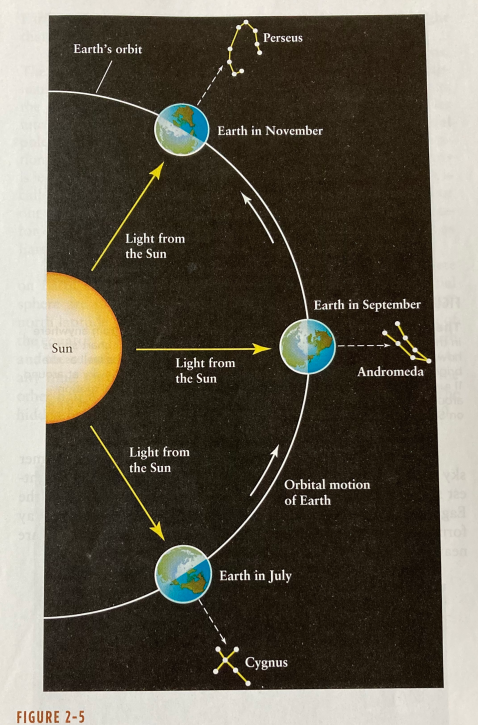
\includegraphics[width=60mm,scale=0.4]{bana.png}
  \caption{Jordbanan mellan Juni och December}
  \label{fig4}
\end{figure}

Om vi bortser från att stjärnor inte kan ses under soljus så ser det ut som, enligt bilden, att Perseus skyms av solen och därmed inte är synlig men frågan
kan inte besvaras om villkoret "stjärnorna ej synliga i dagsljus" tas bort, därför att om en $z$-axel är placerad mot papprets plan
och jordbanan går i papprets plan så skulle Perseus kunna ligga så högt över pappretsplan (högt värde på z-koordinaten)
att man skulle kunna se den ovanför solen.
Nu kan vi dock inte se stärnor som ligger ovanför solen så oavsett Persus värde i $z$ så ser vi inte denna den 15:onde Maj.

\item Hur många grader är zenit från horisonten
och spelar det någon roll var ifrån horisonten man mäter?\\

Zenith är punkten rakt ovanför en observatör på en sfärisk kropp och är alltid 90 grader från horisonten\footnote{\url{https://www.astronomynotes.com/nakedeye/s4.htm}}
Det spelar ingen roll varifrån på horisonten man mäter. Underförstått i begreppet ``horisont'' är att det är en
horisontell rät linje. 

\item Med hjälp av en skiss, förklara hur jordens lutande axel, sett
mot dess omloppsbana kring solen, skapar de årstider vi upplever.\\

Från siten \url{https://media.sciencephoto.com/image/e0900003/800wm/E0900003-Earth_s_orbit_showing_seasons.jpg}
\begin{figure}[H]
\centering
  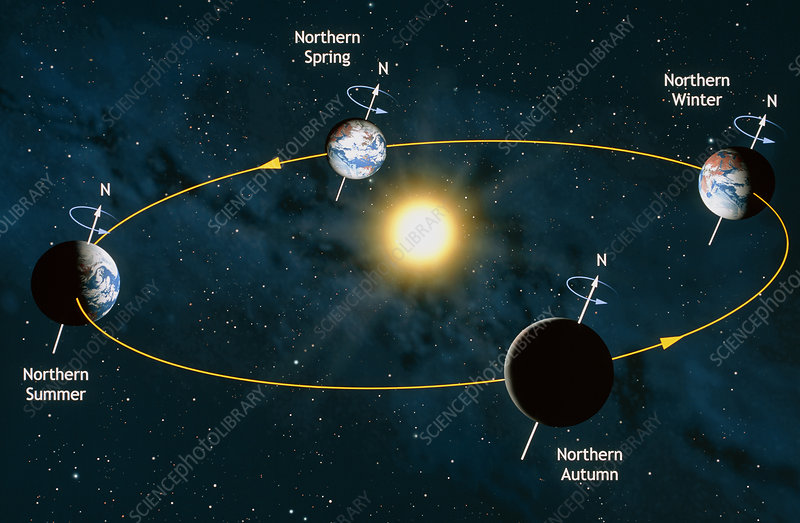
\includegraphics[width=60mm,scale=0.4]{E0900003-Earth_s_orbit_showing_seasons.jpg}
  \caption{Jordens tiltning orsakar årstiderna}
  \label{fig4}
\end{figure}
Vi ser i bilden att projektionsytan för solens strålar är störst på den norra halvklotet i då  jorden har 
positionen längst till vänster i bild p.g.a. dess lutande axel.Lutningen gör att dagen är längst under sommaren för oss på norra
halvklotet och minskar i tid till vintersolståndet varefter dagsljuset ökar i tid. Detta förklarar varför hösten och våren
är varmare än vintern men kallare än sommaren samt det faktum att solstrålarna träffar norra hemisfären i en flackare
vinkel - solen synes inte gå lika högt ovanför os som under sommaren.

\item Ge två anledningar till varför det är varmare på sommaren.\\
Solen är högre ovanför oss och man kan se det som att det är fler strålar per ytenhet som värmer upp jordytan jämfört med då
solljuset kommer in flackare - befinner sig lägre. Vidare tillkommer det faktumet att dagen är längre och därmed integreras
soleffekten under en längre tid under dygnet.

\item Vad är vårdagjämning och höstdagjämning?
Vad är sommar- och vintersolståndet?
Hur relateras dessa fyra punkter till ekliptikan samt ekvatorn?\\

Under vår-och höstdagjämningen är natt och dag lika långa, dagen är som längst under sommarsolståndet och kortast
under vintersolståndet, vilket beror på ekliptikan som är en tänkt solbana i ett koordinatsystem där jorden står still.
Ekliptikan bildar 23.5 grader med ekvatorialplanet.

\item Varför är tiden på ett solur, alltså soltiden, inte nödvändigtvis densamma som på en
analog/dialog klocka?\\

Därför att vi har tidszoner där vi har bestämt att en viss tid skall gälla vilket betyder att när klockan slår exakt 13:00
så behöver detta inte vara soltiden kl. 13:00 i Enköping där jag är bosatt. Soltiden är beroende av den geografiska platsen
på ett kontinuerligt vis.

\item Vad är skillnaden på sidereal tid samt tropisk tid? Varför är dessa två år olika långa? Varför
baseras kalendrarna på det tropiska året?\\

Ett tropiskt år är tiden det tar för solen att återvända till samma position med avseende på andra himlakroppar.
\textit{A tropical year or solar year (or tropical period) is the time that the Sun takes to return to the same position in the sky of a celestial body of the Solar System such as the Earth, completing a full cycle of seasons;}\footnote{\url{https://en.wikipedia.org/wiki/Tropical_year}} 

Ett sidrealt år är tiden för jorden att göra ett varv runt solen med himla kroppar såsom referens.
Ett sidrealt definierat dygn är kortare än ett verkligt dygn s.k. soldygn, se bilden från Wikipedia
\begin{figure}[H]
 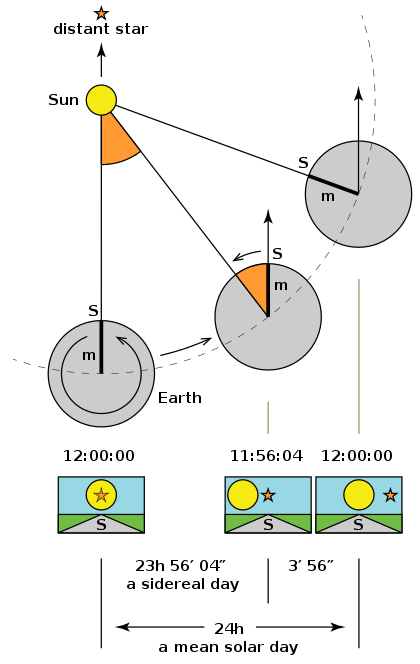
\includegraphics[width=\linewidth]{sidereal.png}
  \caption{Sidrealt dygn jämfört med soldygn. Sidreala beskriver inte en full 360 gradig jordrotation med avseende på solen}
  \label{fig4}
\end{figure}
Detta betyder att om man sidreal dygnsmätning används så måste året bestå av ca 366 dagar.
De tropiska året följer årstiderna därför att det är baserat på solens skenbara rörelse gentemot kroppar såsom jorden.
Hur detta hänger ihop med solur,analemma, precession, Julianska kalendern, Greogianska kalendern, kompensationer vart 400:de år etc.
försöker jag begripa med användandes av youtube därför att jag inte har råd med boken. Det går dock inte särklit bra för mig.






 

\end{enumerate}


%\underbrace{}

% \hspace{1em}

%\begin{enumerate}[label=(\alph*)]
%\end{enumerate}

%$$
%  A = 
%  \begin{bmatrix}
%    1 & 0  & 2i\\
%    2i & 0 &  -4\\
%    -i &  0 & -2i\\
%  \end{bmatrix}
%$$

%\begin{flalign*}
%  A = 
%  \begin{bmatrix}
%    1 & 0  & 2i\\
%    2i & 0 &  -4\\
%    -i &  0 & -2i\\
%  \end{bmatrix}
%\end{flalign*}


%\begin{flalign*}
%\psi(x) = \begin{cases} Ae^{ikx}+Be^{-ikx} &\ \  x<-a \\
%                        Ce^{\kappa x}+De^{-\kappa x} &\ \ -a < x < a\\
%						Fe^{ikx} & \ \ x>a
%       \end{cases}
%\end{flalign*}
%[width=80mm,scale=0.7]
%\begin{figure}[H]
%  \includegraphics[width=\linewidth]{odd_finite.eps}
%  \caption{$z_0=0.1\pi,0.5\pi, 3\pi,7\pi$}
%  \label{fig4}
%\end{figure}
\end{document}












                                     
                                     



